\documentclass{beamer}

\title{Image Steganography with FPGA}
\author{Aithu Snehith, Nakka Chakradhar}
\date{}
\begin{document}

\begin{frame}
\titlepage
\end{frame}

\begin{frame}
	\tableofcontents
\end{frame}

\section{Introduction}
\frame{
\frametitle{Introduction}

STEGANOGRAPHY:
\vspace{5mm} \newline
Steganography is the practice of concealing a file(any information) within another file.

}
\section{Project Scope}
\frame{
\frametitle{Project Scope}

This project is useful for hiding information  in any file.
The scope of the project is implementing steganography on FPGAs for hiding information which includes any type of files like image files, audio files, video, apk etc., in any other file.
\vspace{5mm} \newline
For this project we're hiding a message string in an image file.
}

\section{Methodology}
\frame{
\frametitle{Methodology - LSB insertion}

The LSB is the lowest significant bit in the byte value of the character.
\vspace{5mm} \newline
The LSB based image steganography hides the secret(byte) in the least significant bits of pixel values of the cover image.
\begin{figure}[t!]
    \centering
    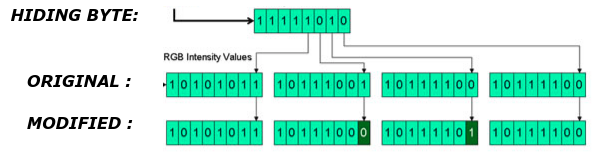
\includegraphics[width=0.6\textwidth]{lsb.png}
    \caption{Overview of LSB Insertion}
\end{figure}
}

\section{Implementation}
\subsection{RISC-V on IcoBoard}
\frame{
\frametitle{RISC-V on IcoBoard}

The RISC-V is an exciting Free and Open Instruction Set architecture. Clifford Wolf (the curator of icotools) has implemented (in verilog), a size-optimized version of the RISC-V architecture called the PicoRV32. It is possible to implement a PicoRV32 processor using the Lattice ICE40 FPGA present on the IcoBoard
}

\subsection{UART and GCC on IcoBoard}
\frame{
\frametitle{UART and GCC on IcoBoard}
With the help of icotools, one can implement a working UART connection. Also, one could write a C code to control the PMOD pins (aka GPIO) on IcoBoard.
\vspace{5mm} \newline
Our idea is to open a port on Raspberry Pi, access a required file and send the bits sequentially to the FPGA where the bits are processed and sent back.
}

\section{Current Progress}
\frame{
\frametitle{Current Progress}

Implemented steganography algorithm in C
\vspace{5mm}\newline
Currently we have achieved sending a string, manipulating it and receiving back using UART.
\vspace{5mm}\newline
Currently we have some clock synchronisation and junk output issues.
}
\frame{
\frametitle{Current Progress}
\begin{figure}[t!]
    \centering
    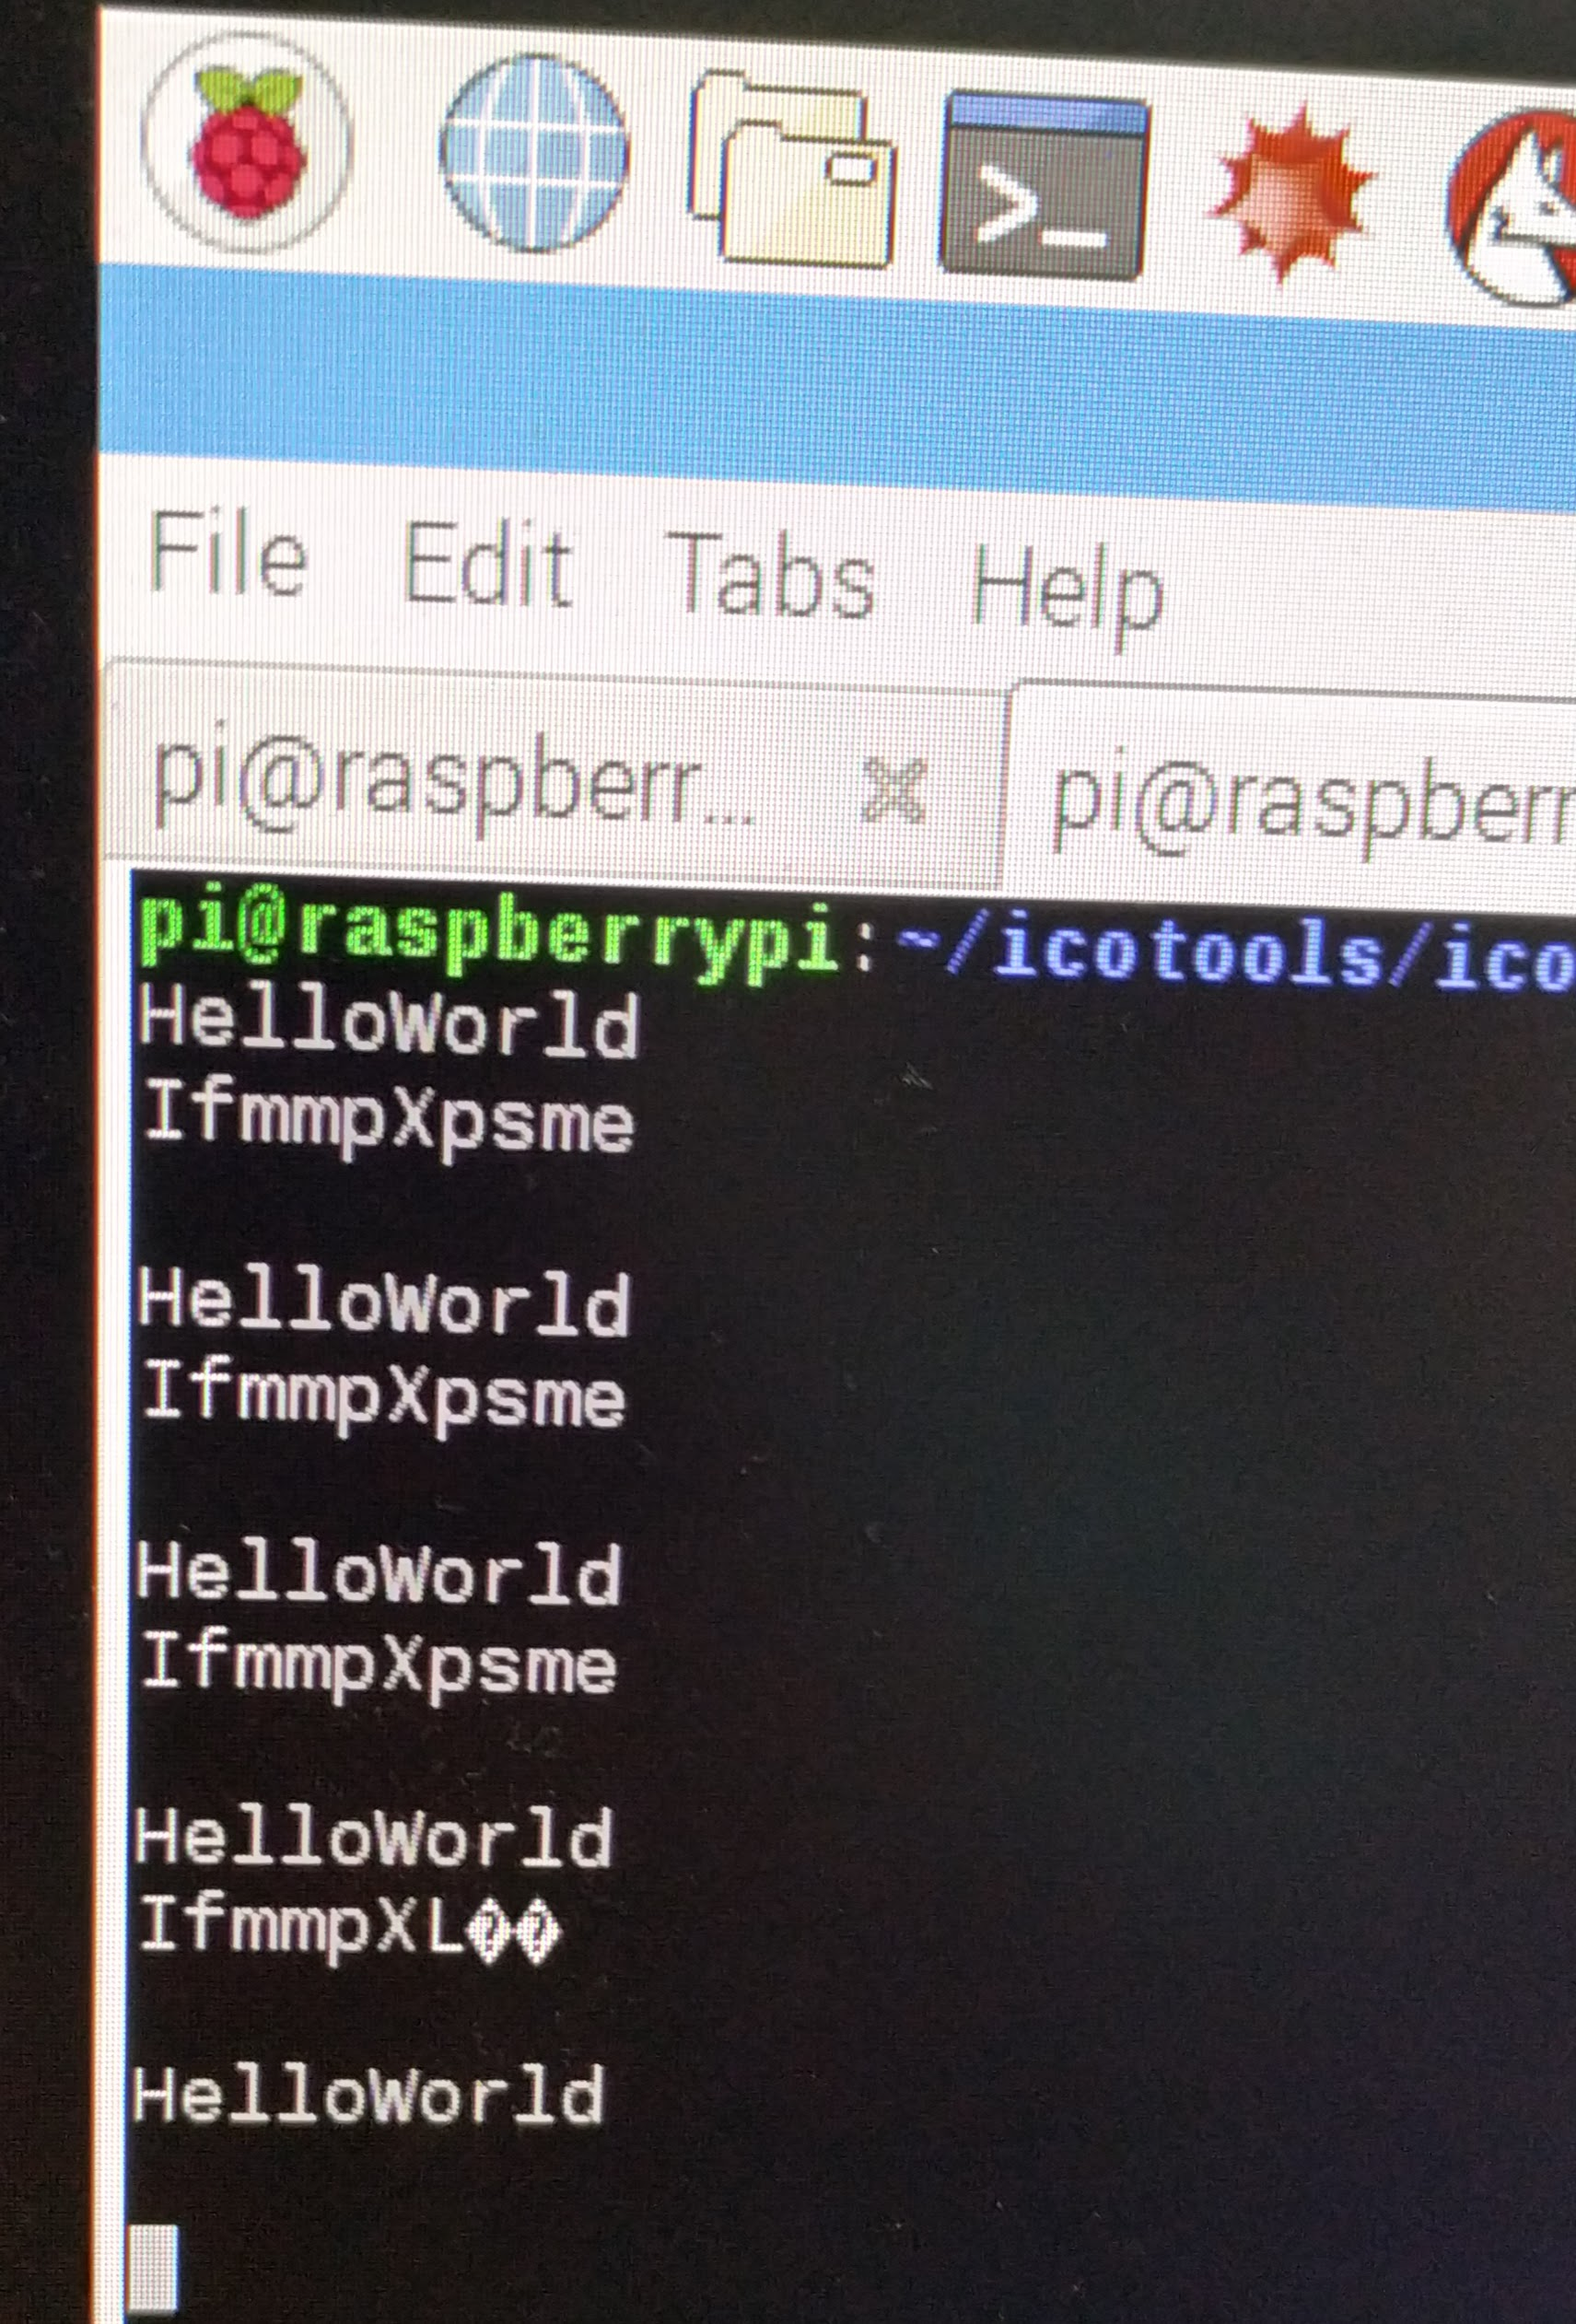
\includegraphics[ height = 200, width=0.6\textwidth]{proof.jpg}
\end{figure}

}

\end{document}
